\chapter{Analyse van Observatieprestaties}
\label{ch:analyse}

\section{Inleiding}

In de voorgaande hoofdstukken werden de ontwikkeling van de PoC applicatie, de methodologie voor het verzamelen 
van experimentele data, en het creëren van een grondwaarheidsdataset uitvoerig besproken. 
Dit hoofdstuk richt zich op de kern van het onderzoek: de geautomatiseerde analyse van de 
observatieprestaties van studenten aan de hand van de verzamelde eyetracking-opnames.

Het hoofddoel van de hier beschreven analyse is, om op basis van de videofeed en blikdata van de Tobii Pro Glasses 3, 
automatisch te bepalen (1) welke van de vooraf gedefinieerde kritische objecten door een student zijn waargenomen en (2) 
hoe lang de aandacht op elk van deze objecten gericht was. 
Om dit te realiseren, werd een analysepipeline ontworpen en geïmplementeerd, die de output van verschillende computervisiemodellen combineert.

De ontwikkelde analysepipeline, zoals conceptueel voorgesteld in Strategie 4 van Hoofdstuk~\ref{ch:oplossingsstrategieen}, 
transformeert de ruwe video- en blikdata, frame-per-frame tot een identificatie van bekeken, kritische objecten. 
Dit proces omvat drie hoofdfasen: (1) het segmenteren en tracken van alle potentiële objecten in beeld, 
(2) het filteren van deze segmenten op basis van objectgrootte en daadwerkelijke observatie door de student, en 
(3) het classificeren van de overgebleven objectsegmenten. 
Er werden drie verschillende benaderingen voor de classificatiestap geëvalueerd:
\begin{enumerate}
  \item \textbf{Vector-Index Classificatie:} Hierbij worden eerst image embeddings van de bekeken segmenten gegenereerd met DINOv2.
  Hierna worden deze embeddings vergeleken met voorbeelden van de kritische objecten binnen een \texttt{Faiss (Facebook AI Similarity Search)} vector-index.
  \item \textbf{YOLOv11 Classificatie:} In deze benadering wordt een YOLOv11-model getraind om de segmenten te classificeren.
  \item \textbf{YOLOv11 Object Detectie:} Deze aanpak verschilt van de vorige doordat het model niet enkel classificeert, 
  maar ook de locatie van de objecten in het frame bepaalt. 
  De objectdetector genereert bounding boxes, die vervolgens worden gecombineerd met de trackingresultaten van FastSAM om tot een definitieve classificatie te komen van elk bekeken object.
\end{enumerate}
Merk op dat het bij de eerste fase niet enkel over frame-per-frame segmentatie gaat, maar ook over het tracken van deze segmenten doorheen de video.
Deze aanpak maakt het mogelijk om na classificatie van de individuele segmenten, de resultaten te aggregeren over de volledige tracking-sessie van elk object. 

De ontwikkelde methoden werden beoordeeld aan de hand van de in Hoofdstuk~\ref{ch:grondwaarheid} gecreëerde grondwaarheid.

Figuur~\ref{fig:analyse-pipeline-visualisatie} illustreert de fasen van dit proces aan de hand van illustratieve beelden.

\begin{figure}[H]
    \centering
        \begin{subfigure}[b]{0.75\textwidth}
        \centering
        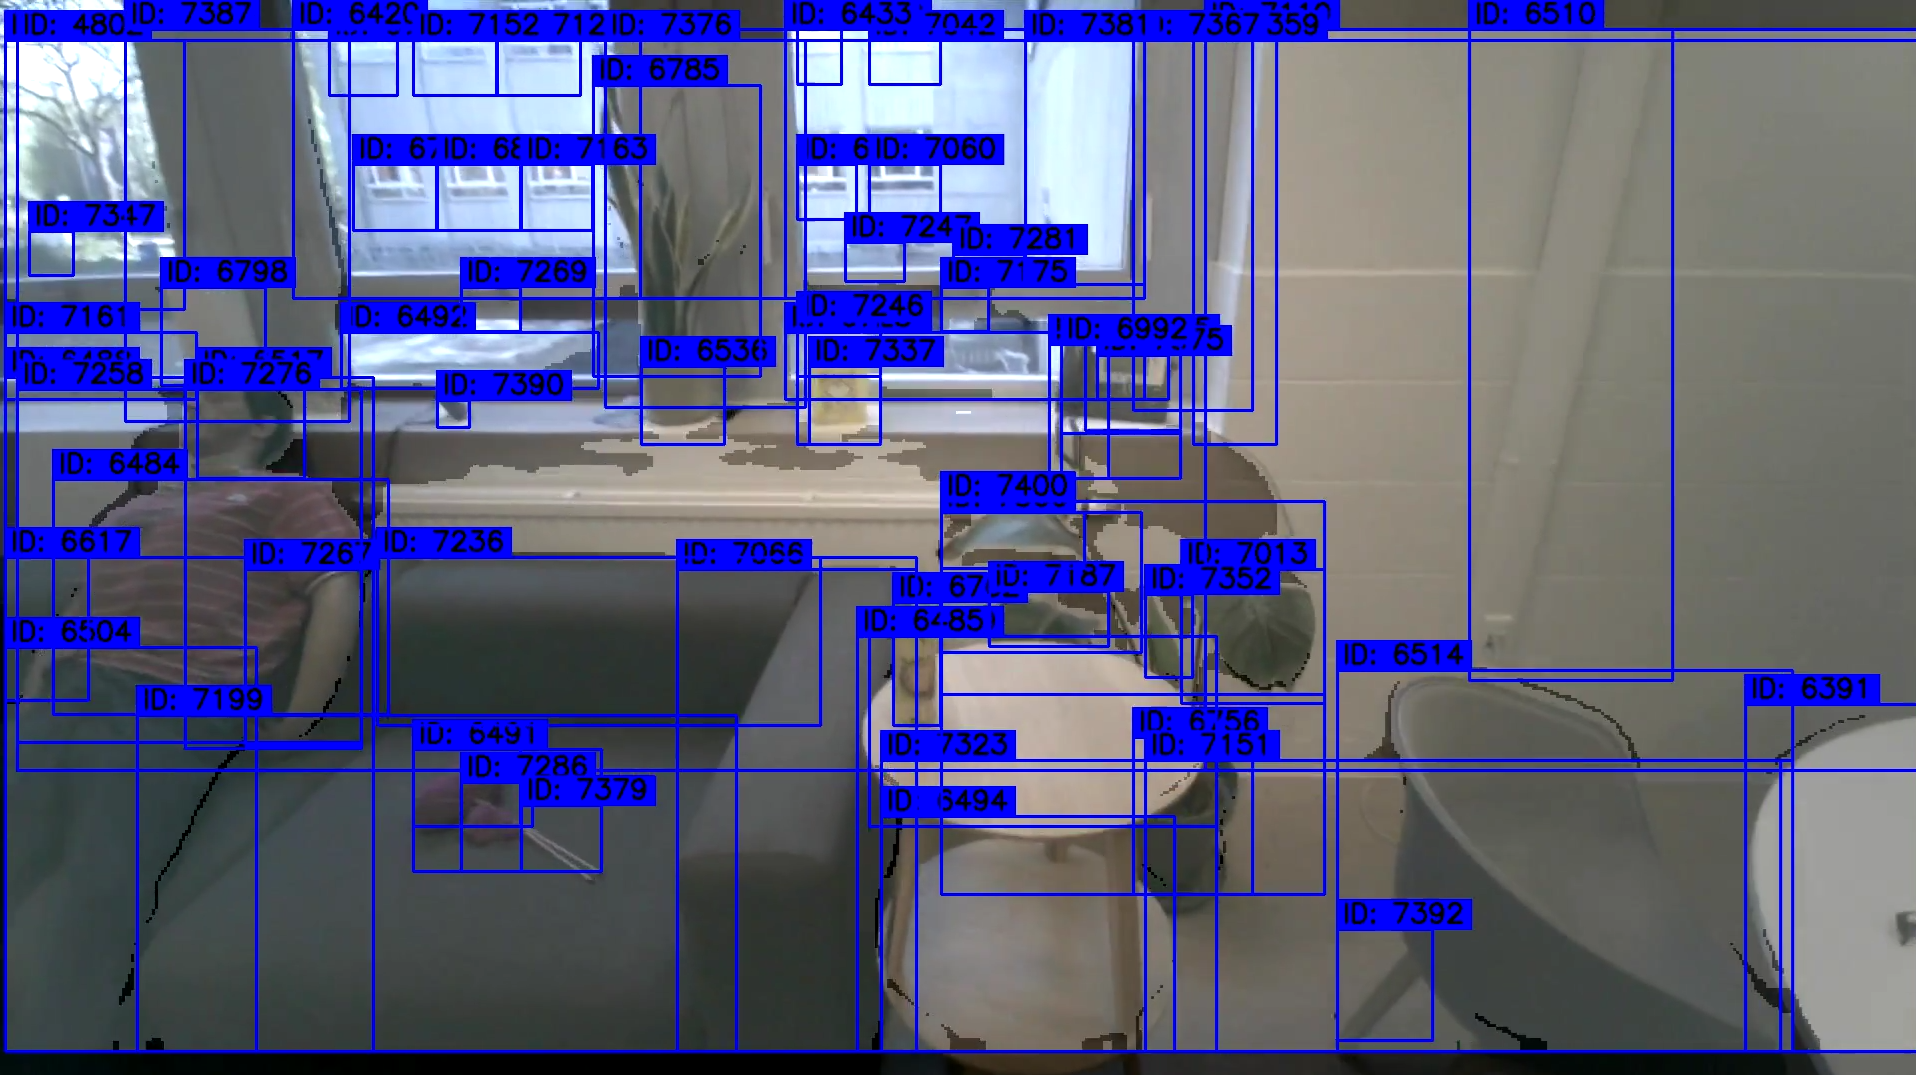
\includegraphics[width=1\textwidth]{everything-prompt.png}
        \caption{Everything-Segmentatie (FastSAM)}
        \label{fig:pipeline_stap_a}
    \end{subfigure}

    \vspace{0.5cm}

    \begin{subfigure}[b]{0.75\textwidth}
    \centering
    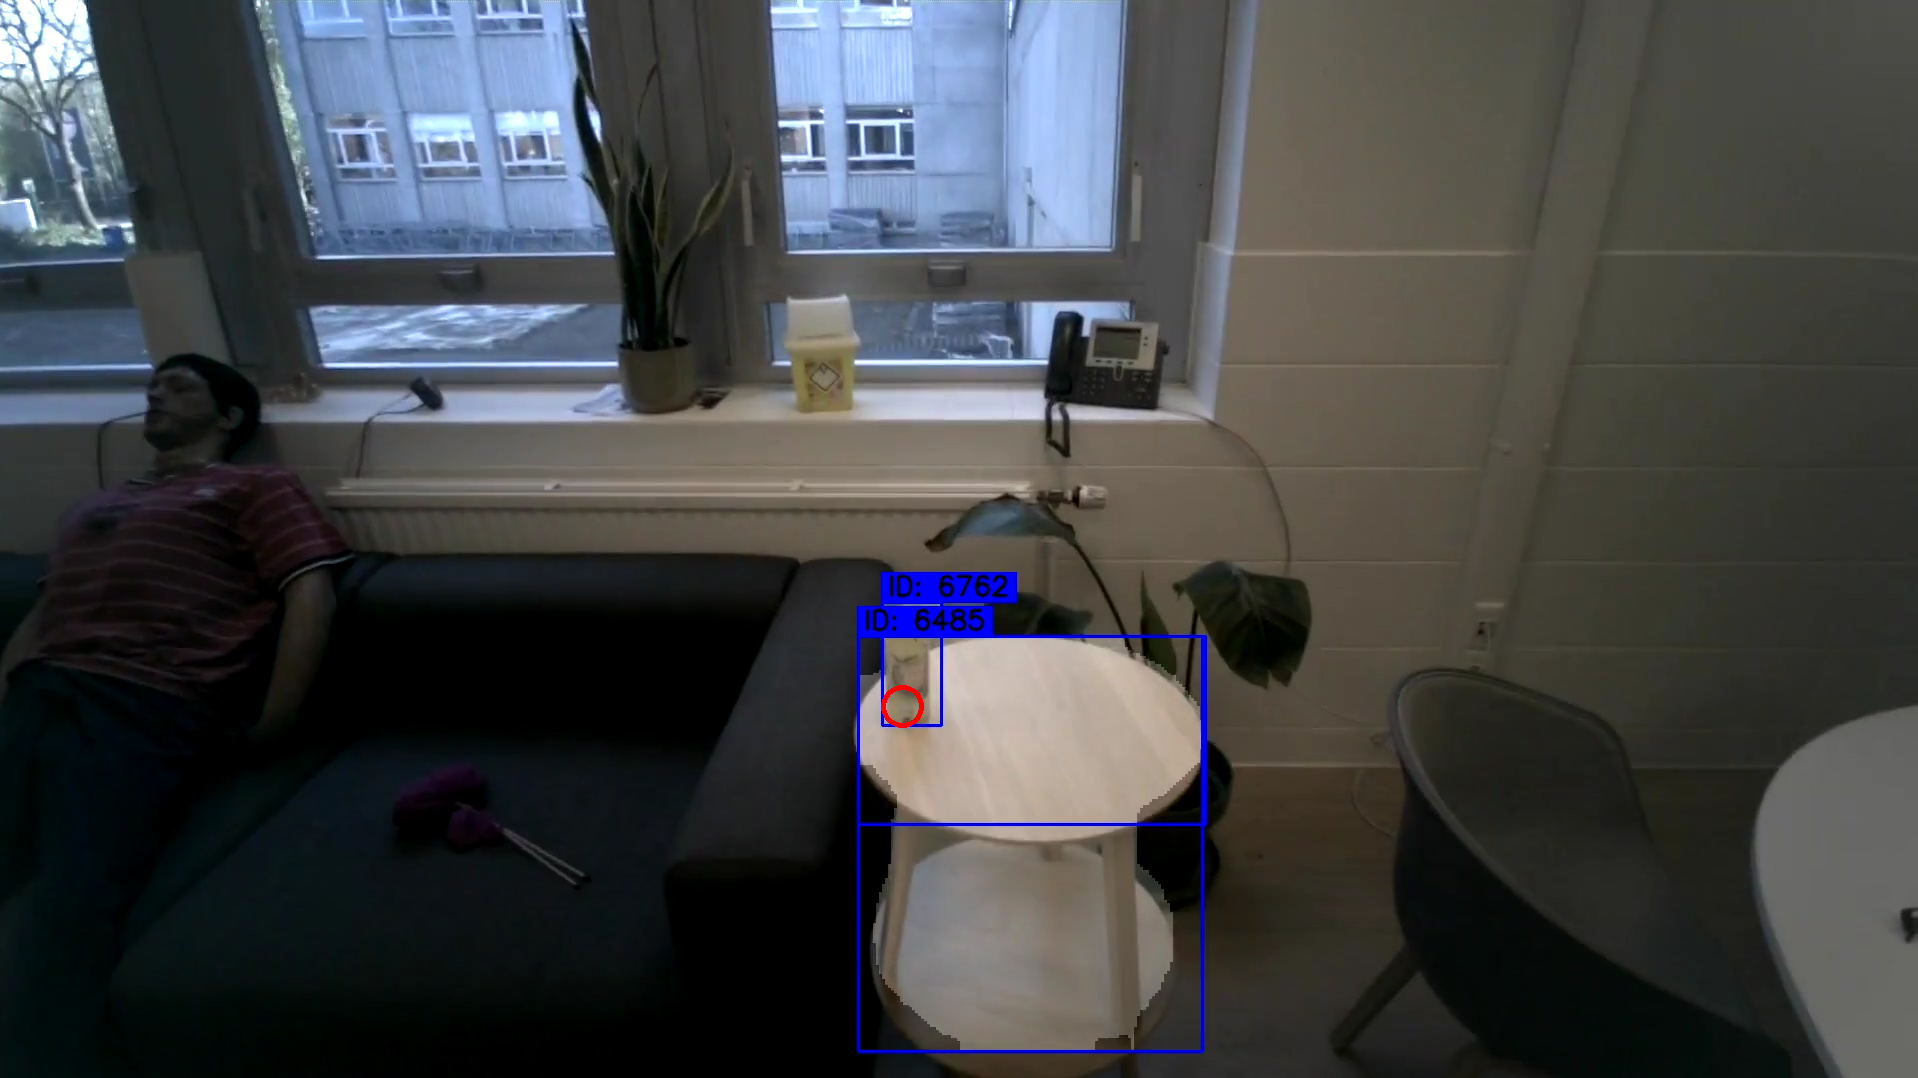
\includegraphics[width=1\textwidth]{filtered-segmentation.png}
    \caption{Filtering op basis van blikpunt en objectgrootte}
    \label{fig:pipeline_stap_b}
    \end{subfigure}

    \vspace{0.5cm}

    \begin{subfigure}[b]{0.75\textwidth}
        \centering
        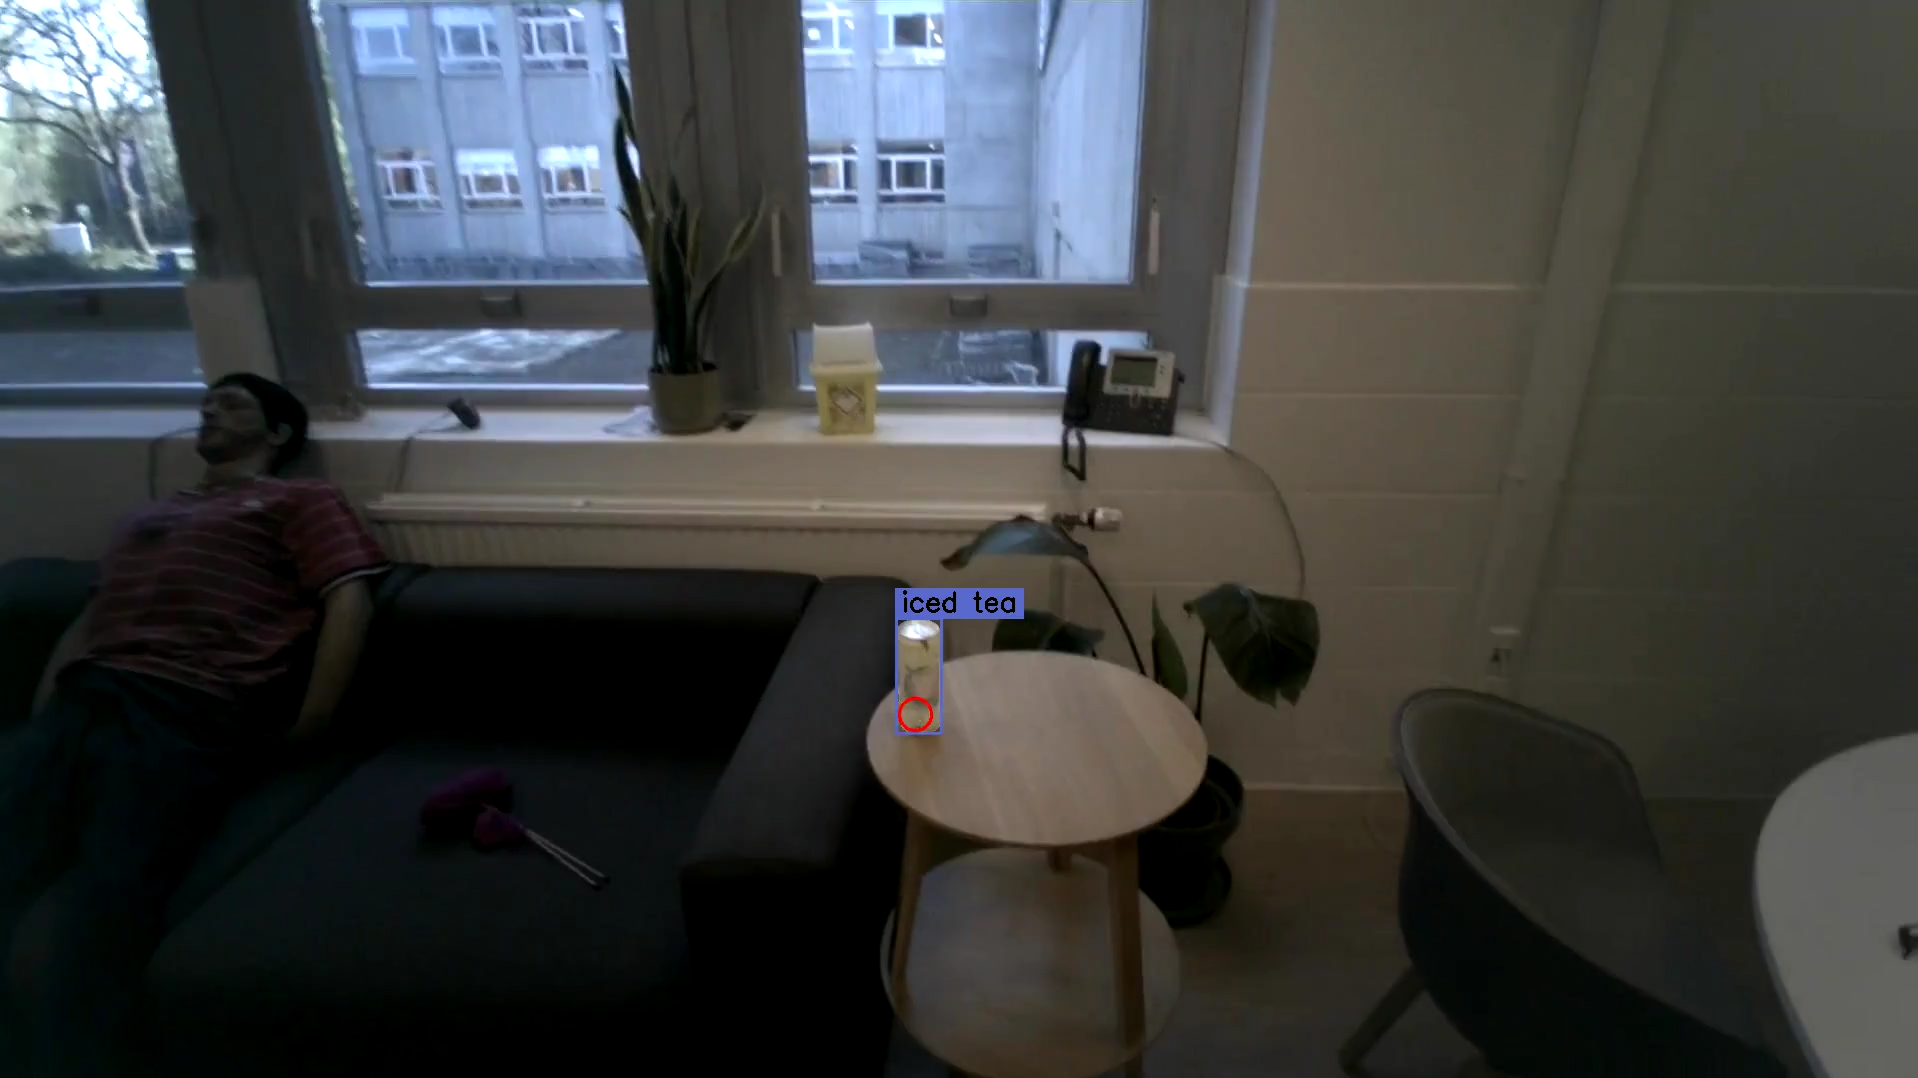
\includegraphics[width=1\textwidth]{classification-example.png}
        \caption{Classificatiestap}
        \label{fig:pipeline_stap_c}
    \end{subfigure}
    \caption[Visualisatie van de Analysepipeline]{
        \label{fig:analyse-pipeline-visualisatie}
        Visualisatie van de stappen in de analysepipeline.
        (\subref{fig:pipeline_stap_a}) FastSAM segmenteert alle objecten in het beeld en volgt deze doorheen de video.
        (\subref{fig:pipeline_stap_b}) De segmenten worden gefilterd; enkel de segmenten die daadwerkelijk met de blik van de gebruiker overlappen worden behouden.
        (\subref{fig:pipeline_stap_c}) De overgebleven segmenten worden uit de originele frame geknipt en dienen als input voor een classificatiemodel.
    }
\end{figure}

\section{Tracking en Segmentatie van Objecten}
\label{sec:tracking-segmentatie}

De eerste fase van de analysepipeline is erop gericht om uit de continue videostroom alle potentieel relevante objectregio's 
te isoleren die daadwerkelijk door de student zijn bekeken. 
De implementatie van dit proces werd vastgelegd in de python-notebook \texttt{04\_gaze\_segmentation.ipynb},
en wordt hieronder toegelicht.
De besproken code binnen deze fase is terug te vinden in de \texttt{GazeSegmentationJob} klasse in de notebook.

Voor deze fase werd gekozen om gebruik te maken van het FastSAM-model, vanwege zijn hoge snelheid.
Dit maakte het mogelijk om snel de aanpak te optimaliseren en de pipeline te testen, zonder dat de tijdsduur van de analyse een beperkende factor werd.
Het model komt in twee varianten: een `large' (\texttt{FastSAM-x}) en een `small' (\texttt{FastSAM-s}) versie.
Er werd gekozen om de `large' versie te gebruiken, vanwege de betere segmentatiekwaliteit.
FastSAM is beschikbaar via de \texttt{ultralytics}\footnote{\url{https://docs.ultralytics.com/models/fast-sam/} (laatst geraadpleegd op 2025-05-21)} python-bibliotheek,
die een \texttt{track} functie bevat die het mogelijk maakt om alle objecten in een video zowel te segmenteren als te tracken.

\subsection{Tracking en Segmentatie van Objecten}

In een eerste stap worden alle frames van de evaluatieopname geëxtraheerd naar een tijdelijke map met behulp van \texttt{ffmpeg}.
Daarna is het mogelijk om de \texttt{track} functie toe te passen op deze frames:

\begin{listing}[H]
  \begin{minted}{python}
    frame_paths = list(self.frames_path.iterdir())
    # Frames sorteren op basis van hun naam (index)
    frame_paths.sort(key=lambda x: int(x.stem))

    for frame_path in frame_paths:
        frame_idx = int(frame_path.stem)
        results = self.model.track(
            source=str(frame_path), imgsz=1024, verbose=False, persist=True
        )[0]
    \end{minted}
  \caption[Tracking van objecten met FastSAM]{}
\end{listing}

Hier zijn volgende zaken belangrijk om op te merken:
\begin{itemize}
    \item De frames dienen gesorteerd te worden op basis van hun volgorde in de video.
    \item De \texttt{track} functie neemt een parameter \texttt{imgsz} aan, die de grootte van de inputafbeeldingen bepaalt.
    Indien de afbeeldingen te groot of te klein zijn, worden ze automatisch geschaald.
    Deze parameter heeft zowel invloed op de snelheid van de segmentatie als op de kwaliteit ervan.
    \item Het is belangrijk om de \texttt{persist} parameter op \texttt{True} te zetten, 
    zodat het model de tracking-informatie kan behouden tussen opeenvolgende frames.
    \item De \texttt{track} functie levert een lijst op van \texttt{Results}-objecten, maar bevat hier slechts één element, aangezien de functie telkens een enkele frame behandelt.
    Dit \texttt{Results}-object bevat de segmentatiemaskers, bounding boxes, en tracking-informatie voor elk object in het frame.
\end{itemize}

% TODO: IOU? CONF?

\subsection{Filteren van Tracking-Resultaten}

Na het uitvoeren van de tracking en segmentatie, worden de resultaten gefilterd op basis van twee criteria:
\begin{itemize}
    \item \textbf{Objectgrootte:} Segmenten die een onrealistisch groot deel van het beeld beslaan (bijvoorbeeld muren, vloeren, of de gehele achtergrond) worden weggelaten.
    \item \textbf{Blikdata:} Met behulp van de \texttt{mask\_was\_viewed} functie (zie Sectie~\ref{sec:filtering-annotaties}) 
    wordt voor elk overgebleven segment gecontroleerd of het blikveld van de student daadwerkelijk overlapt met het segmentatiemasker in dat specifieke frame. 
    Enkel de `bekeken' segmenten worden behouden voor verdere analyse.
\end{itemize}

Hier zullen we enkel de \texttt{mask\_too\_large} functie toelichten.
Codefragment~\ref{listing:filteren-segmenten-grootte} toont de implementatie hiervan.

\begin{listing}[H]
  \begin{minted}{python}
    def mask_too_large(self, mask: torch.Tensor) -> bool:
        MAX_MASK_AREA = 0.1
        height, width = mask.shape
        frame_area = height * width
        max_mask_area = MAX_MASK_AREA * frame_area

        mask_area = mask.sum()
        return mask_area >= max_mask_area
    \end{minted}
  \caption[Filteren van segmenten op basis van grootte]{
    \label{listing:filteren-segmenten-grootte}  
    Deze functie controleert of een segment te groot is op basis van de oppervlakte van het segmentatiemasker. 
  }
\end{listing}

Hier wordt een som berekend van alle pixels in het segmentatiemasker (aangezien het masker binair is).
Indien deze som groter is dan de maximaal toegestane oppervlakte, wordt het masker als `te groot' beschouwd.
De maximale oppervlakte van een segment wordt gedefinieerd als 10\% van de totale oppervlakte van het frame.
Dit is momenteel een arbitraire waarde, maar kan in de toekomst verder geoptimaliseerd worden, of zelfs 
dynamisch worden ingesteld op basis van objecten binnen kalibratieopnames in de applicatie.

\subsection{Opslaan van de Resultaten}

Na het filteren van de segmenten, worden de resultaten van elke frame opgeslagen in gecomprimeerde numpy-bestanden 
(\texttt{.npz}) onder \texttt{data/gaze\_segmentation\_results}.

\begin{listing}[H]
  \begin{minted}{python}
    executor.submit(
        np.savez_compressed,
        self.results_path / f"{frame_idx}.npz",
        boxes=boxes,
        rois=rois_array,
        masks=masks_array,
        object_ids=object_ids,
        frame_idx=frame_idx,
        gaze_position=gaze_position,
        confidences=confidences,
    )
    \end{minted}
  \caption[Opslaan van segmentatie-resultaten]{
    \label{listing:opslaan-segmentatie-resultaten}
    Deze code slaat de resultaten van de segmentatie en tracking op in een gecomprimeerd numpy-bestand.
    De resultaten worden opgeslagen per frame, met de relevante metadata.
  }
\end{listing}

De volgende gegevens worden opgeslagen:
\begin{itemize}
    \item \textbf{boxes:} De bounding boxes van de segmenten, handig voor het visualiseren van de segmenten in de video.
    \item \textbf{rois:} De ROI's (Region of Interest) van de segmenten. Deze worden later gebruikt bij de classificatiestap om de objecten te identificeren.
    \item \textbf{masks:} De segmentatiemaskers van de objecten, die ook worden gebruikt voor visualisatie.
    \item \textbf{object\_ids:} De unieke ID's van de objecten, die worden toegewezen door het FastSAM-model. Deze ID's blijven consistent voor elk specifiek object over meerdere frames,
    tenzij de tracking verloren gaat (bijvoorbeeld wanneer het object tijdelijk uit beeld is). Wanneer dit gebeurt, wordt een nieuwe ID toegewezen aan het object als het opnieuw in beeld komt.
    Deze ID maakt het mogelijk om de resultaten van de classificatiestap te aggregeren over meerdere frames, om zo een beter resultaat te krijgen.
    \item \textbf{frame\_idx:} De index van het frame, die wordt gebruikt om de resultaten te koppelen aan het juiste frame in de video.
    \item \textbf{gaze\_position:} De blikpositie van de student in dat specifieke frame (indien beschikbaar).
    \item \textbf{confidences:} De vertrouwensscore van het model voor elk segment, die aangeeft hoe zeker het model is dat het segment correct is.
    Dit kan nuttig zijn voor het filteren van segmenten die een lage vertrouwensscore hebben, 
    of het vinden van correlaties tussen de vertrouwensscore en de uiteindelijke classificatie.
\end{itemize}
Aangezien het opslaan van de resultaten IO-intensief is, wordt dit proces uitgevoerd met behulp van multithreading (\texttt{executor.submit}).

\subsection{Voorbereiding van de Tracking Resultaten voor Classificatie}
\label{sec:voorbereiding-tracking-resultaten}

De output van de vorige stap bestaat uit een reeks \texttt{.npz}-bestanden, één per frame, 
die de gefilterde segmenten, ROIs, en bijbehorende metadata bevatten. 
Om deze data efficiënt te kunnen gebruiken als input voor de classificatiestrategieën, werd een aanvullende voorbereidingsstap uitgevoerd. 
Deze stap werd geïmplementeerd in de notebook \texttt{05\_create\_object\_datasets.ipynb} en consolideert de frame-per-frame 
resultaten tot een gestructureerde dataset per evaluatieopname. 
Deze dataset, hierna `object-dataset' genoemd, aggregeert alle metadata van de bekeken segmenten binnen een enkele tabel.
Hoewel veel van deze metadata ook in de individuele \texttt{.npz}-bestanden te vinden zijn, resulteert de consolidatie 
naar één \texttt{.csv}-bestand per opname in een efficiëntere dataverwerking tijdens de classificatiefase. 
Het vermijdt het herhaaldelijk openen en parsen van potentieel honderden of duizenden afzonderlijke \texttt{.npz}-bestanden.

Het creëren van de object-dataset omvat het itereren over de \texttt{.npz}-bestanden van elke opname. 
Voor elk gedetecteerd en gefilterd object (ROI) binnen een frame worden de volgende kenmerken geëxtraheerd en samengevoegd tot een rij in een \texttt{Pandas DataFrame}:
\begin{itemize}
    \item \texttt{frame\_idx}: De index van het frame waarin het object oorspronkelijk werd gedetecteerd. 
    Dit koppelt het object aan een specifiek tijdstip in de video.
    \item \texttt{object\_id}: De unieke, tijdelijke ID die door het FastSAM-model aan het getrackte object 
    is toegewezen binnen de scope van die specifieke tracking-sessie.
    \item \texttt{confidence}: De vertrouwensscore van het FastSAM-model voor de detectie van dit specifieke segment. 
    Deze score geeft een indicatie van hoe zeker het model was van zijn segmentatie.
    \item \texttt{embedding}: Een dense vectorrepresentatie (embedding) van de visuele kenmerken van de ROI, 
    gegenereerd met het DINOv2-model. 
    Deze embedding dient als input voor de op similariteit gebaseerde classificatie met een vector-index.
    Meer hierover in de volgende sectie.
    \item \texttt{mask\_area}: De totale oppervlakte van het segmentatiemasker van het object in pixels. 
    Dit geeft een maat voor de (schijnbare) grootte van het object in het frame.
    \item \texttt{x1, y1, x2, y2}: De coördinaten die de bounding box rondom het gedetecteerde object definiëren. 
\end{itemize}

De resulterende \texttt{DataFrame} wordt vervolgens opgeslagen 
als een \texttt{.csv}-bestand onder \texttt{data/object\_datasets/<recording\_id>}. 
Het resultaat is een set van tabelvormige datasets die klaar zijn voor de daadwerkelijke classificatietaken.

\section{Classificatie van Objecten}

De vorige fase leverde een dataset op met bekeken objectsegmenten (ROIs) per evaluatieopname.
Deze kregen echter nog geen label toegewezen, dat aangeeft tot welk van de kritische objecten ze behoren.
Om dit te realiseren, werd een classificatiestap geïmplementeerd die de ROIs labelt op basis van hun visuele kenmerken.

\subsection{Data Labeling}

Voor het initialiseren en trainen van de classificatiestrategieën was het noodzakelijk om een dataset te hebben met gelabelde objecten.
Zoals eerder beschreven in Hoofdstuk~\ref{ch:experiment} (Sectie~\ref{sec:kalibratieopnames}), werden hiertoe 
twee specifieke kalibratieopnames gemaakt door de onderzoeker.
De eerste opname bevatte de objecten in hun oorspronkelijke posities en achtergrond, identiek aan de evaluatieopnames.
De tweede opname toonde dezelfde objecten tegen een significant afwijkende achtergrond, 
primair bedoeld om de invloed van contextvariatie te onderzoeken.

Bij de analyses die in dit hoofdstuk worden gepresenteerd, is uitsluitend gebruik gemaakt 
van de data uit de kalibratieopname met de originele achtergrond.
De beslissing om de tweede kalibratieopname buiten beschouwing te laten, werd genomen om de scope van deze bachelorproef beheersbaar te houden.
Een discussie over het potentieel van deze tweede dataset voor verder onderzoek is terug te vinden in Hoofdstuk~\ref{ch:conclusie}.
% TODO: toevoegen aan conclusie

\paragraph{Labeling voor Classificatie}
Voor de initiële, op ROI-gebaseerde classificatiepogingen, was de labelingstrategie relatief eenvoudig.
Het volstond om voor elk van de objecten een representatief aantal ROIs te verzamelen en te labelen gedurende de 
tijdsvensters van 30 seconden waarin elk object centraal werd bekeken. 
Dit leverde voldoende voorbeelden van elk object op voor het trainen van de classificatiemodellen.

\paragraph{Labeling voor Objectdetectie}
Voor het trainen van het objectdetectiemodel was echter een meer omvattende aanpak vereist.
In tegenstelling tot ROI-classificatie die op geïsoleerde objectsegmenten werkt, wordt een objectdetector 
getraind om objecten te lokaliseren binnen een breder beeld.
Tijdens de training analyseert het model `crops' (vierkante regio's van het beeld) en leert het model om objecten te detecteren binnen zulke regio's.
Hierbij is het belangrijk dat binnen de labeling alle objecten in het beeld worden gemarkeerd, die potentieel binnen een crop kunnen vallen
(zie Figuur~\ref{fig:voorbeeld_crop_yolo_training} voor een conceptuele visualisatie van een crop).
De manier waarop deze crops worden gedefinieerd binnen de trainingsdataset, komt later in dit hoofdstuk aan bod.
% TODO: verwijzen naar sectie

\begin{figure}[H]
    \centering
    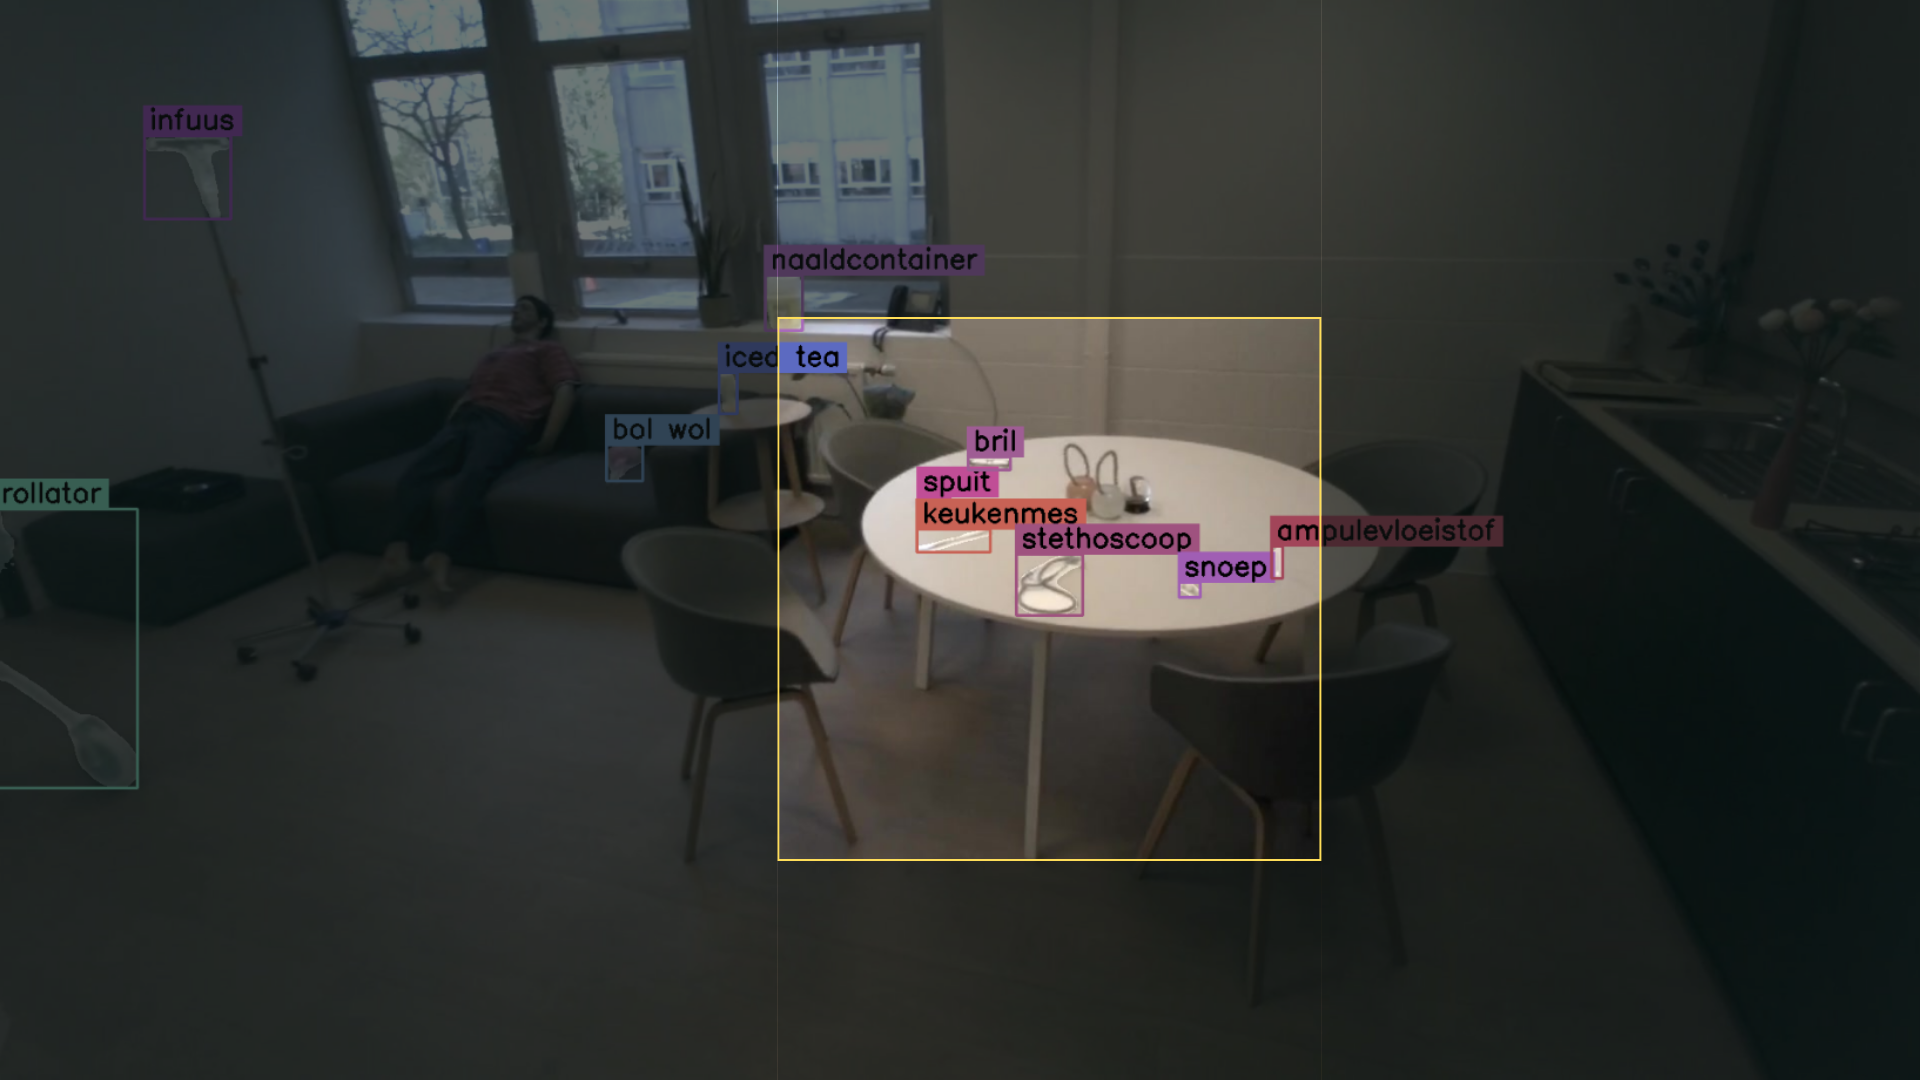
\includegraphics[width=1\textwidth]{yolo_training_crop.png}
    \caption[Voorbeeld van een crop voor objectdetectie]{
        \label{fig:voorbeeld_crop_yolo_training}
        Voorbeeld van een frame uit de labeling tool. 
        Hier wordt een voorbeeld van een crop getoond die gebruikt kan worden voor het trainen van een objectdetectiemodel.
        Het is dus belangrijk dat alle objecten die binnen deze crop kunnen vallen,
        worden gelabeld, zelfs als ze niet volledig zichtbaar zijn.
        Merk op dat dit niet de enige mogelijke crop is binnen deze afbeelding, men kan ook andere regio's selecteren met andere objecten.
    }
\end{figure}

\paragraph{Opmerking: Ampule Poeder Niet Gelabeld}
Het object `ampule poeder' werd in de labeling niet opgenomen. 
Origineel werd het object gekozen omwille van zijn doorschijnende karakter (glazen ampule).
Het werd ook naast een andere groep objecten geplaatst om de detectie alsnog te bemoeilijken (zie Figuur~\ref{fig:ampulepoeder}).
Echter, tijdens de labeling bleek het object te moeilijk voor het SAM2 model om te segmenteren en te tracken.
Dit resulteerde in een lage labelingkwaliteit, waarbij de segmenten inaccuraat waren.
Soms werden zelfs ook foutief aangrenzende objecten meegenomen in de segmentaties.
Om deze reden werd besloten om het object niet mee te nemen in de labeling en de uiteindelijke analyse. 
Een ander object, de `ampule vloeistof', werd wel opgenomen ondanks zijn sterk doorschijnende karakter.
Dit object bleek veel gemakkelijker te volgen en te segmenteren door het FastSAM-model, vermoedelijk omdat het afgezonderd was van andere, 
potentieel verwarrende objecten.

\begin{figure}[H]
    \centering
    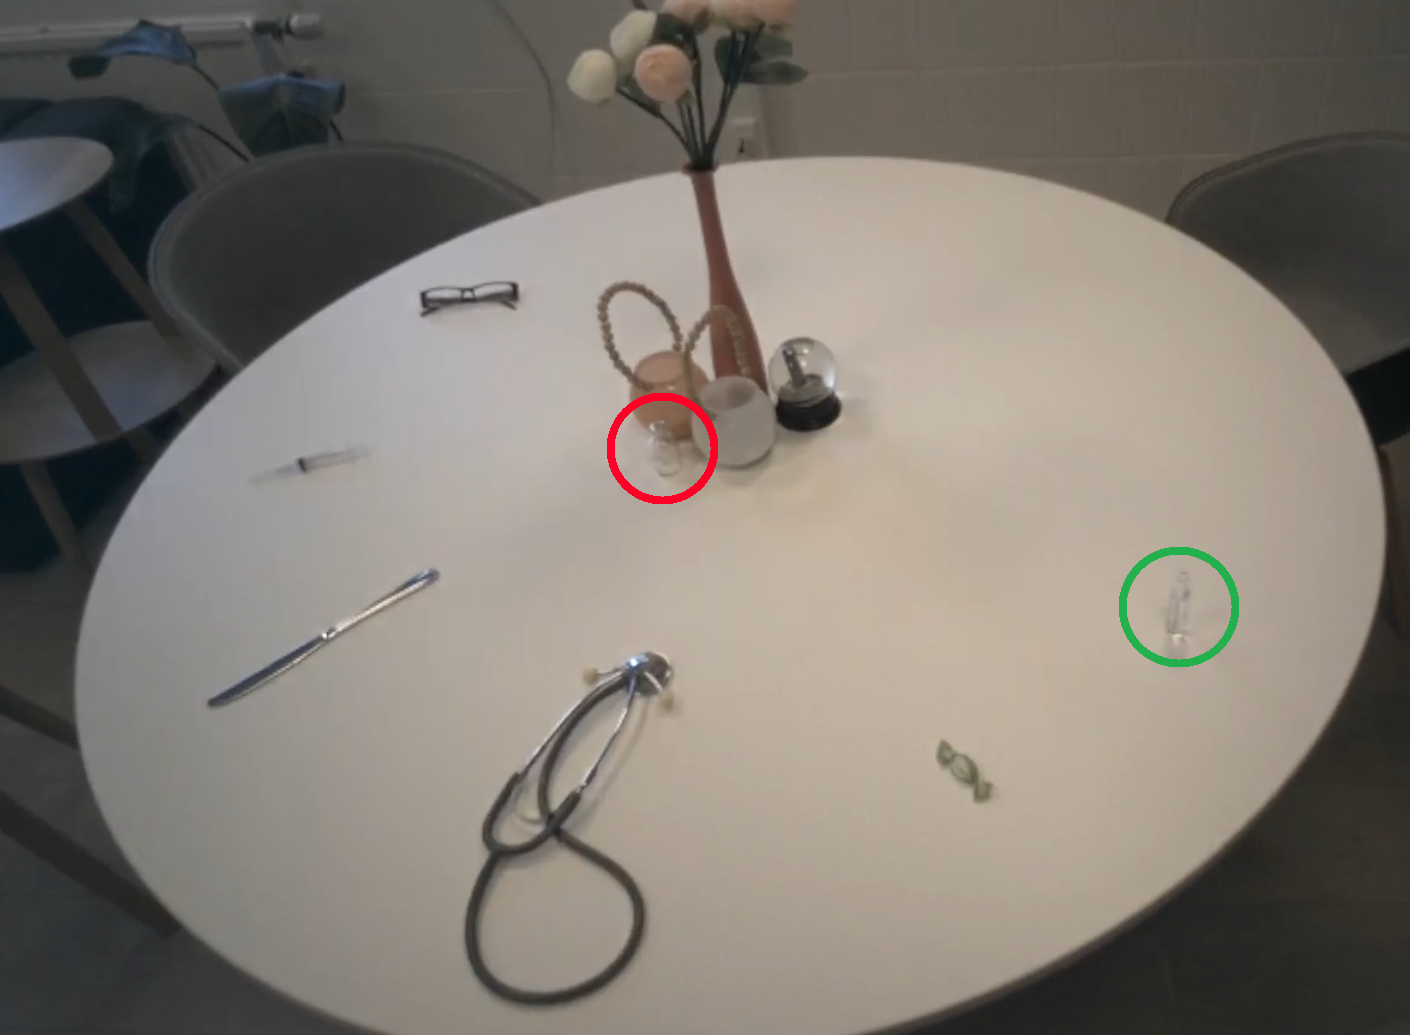
\includegraphics[width=0.8\textwidth]{ampulepoeder.png}
    \caption[Voorbeeld van de ampule poeder in de kalibratieopname]{
        \label{fig:ampulepoeder}
        Locatie van de ampule poeder in de kalibratieopname, aangeduid met een rode cirkel.
        De ampule vloeistof werd wel opgenomen in de labeling, en is hier aangeduid met een groene cirkel.
    }
\end{figure}

\subsection{Initiële Classificatiepogingen en Uitdagingen}

Nadat de object-datasets waren aangemaakt en de referentiedata uit de kalibratieopname was gelabeld, was de volgende stap het 
toewijzen van een label aan elk gedetecteerd en door de student bekeken objectsegment (ROI). 
Er werden initieel twee strategieën onderzocht voor het classificeren van deze ROIs, waarvan de relevante data beschikbaar waren in de object-datasets:
\begin{enumerate}
    \item \textbf{Vector-Index Classificatie:} Hierbij werden de DINOv2-embeddings van de ROIs vergeleken met referentie-embeddings van de kritische objecten afkomstig uit de kalibratieopname.
    Er werd een Faiss (Facebook AI Similarity Search) index gebruikt om de meest vergelijkbare referentie-embeddings te vinden.
    Faiss is een bibliotheek die het mogelijk maakt om snel zoekopdrachten uit te voeren op grote datasets van vectoren.
    \item \textbf{YOLOv11 Classificatie:} Een YOLO-model werd getraind, niet voor detectie in het volledige frame, maar specifiek voor het classificeren van de reeds 
    geïsoleerde ROIs uit de evaluatieopnames.
\end{enumerate}

Deze twee benaderingen zullen hier echter niet diepgaand worden behandeld, 
aangezien beiden al in een vroeg stadium van evaluatie een fundamenteel gebrek vertoonden, 
namelijk een onacceptabel hoge mate van vals-positieven. 
Het probleem lag niet zozeer in de specifieke modelkeuzes, maar in een verkeerde definitie van het classificatieprobleem.
De gekozen classificatietechnieken zijn inherent ontworpen voor \textit{gesloten-set} scenario's. 
In dergelijke scenario's  wordt aangenomen dat elke te classificeren input (elke bekeken ROI)
daadwerkelijk tot één van de vooraf gedefinieerde klassen behoort. 

De realiteit van de observaties is echter complexer en sluit veel beter aan bij het concept van \textit{Open Set Recognition (OSR)}. 
Zoals \textcite{Geng2018} beschrijven in hun overzichtsartikel, is het 
``doorgaans moeilijk om, wanneer men een herkenner of classificator traint, trainingsvoorbeelden te verzamelen die alle (mogelijke) klassen omvatten''.
OSR beschrijft een scenario waarin 
``er ten tijde van de training onvolledige kennis van de wereld bestaat, en onbekende klassen tijdens het testen aan een algoritme kunnen worden voorgelegd''.
Dit vereist dat een classificatiemodel ``niet alleen de geziene klassen accuraat classificeert, maar ook effectief omgaat met de ongeziene'' (citaten uit \textcite{Geng2018}, eigen vertaling).

In de context van dit onderzoek betekende dit dat de studenten talloze objecten en achtergrondelementen bekeken die \textit{niet} tot de kritische objecten behoorden.
De geïmplementeerde ROI-classificatiemodellen waren niet in staat om deze `onbekende' inputs effectief te herkennen en te verwerpen.
In plaats daarvan waren ze geneigd elke ROI te classificeren als één van de objecten, wat resulteerde in de waargenomen overvloed aan vals-positieven.

Gezien deze mismatch tussen de aard van het probleem en de gekozen aanpak, werd besloten deze classificatiestrategieën niet verder te optimaliseren.
De focus verschoof naar een methode die beter is uitgerust om specifieke, bekende objecten te identificeren: objectdetectie.

\section{Objectdetectie met YOLOv11} 

Bij de voorgaande classificatiestrategieën lag de focus op het classificeren van geïsoleerde objectsegmenten afkomstig uit de FastSAM everything-segmentatie.
% TODO: Intro iets beter maken

\subsection{Creatie van de Trainingsdataset voor Objectdetectie}

Gebaseerd op de gelabelde kalibratieopname die eerder werd besproken, werd een specifieke trainingsdataset voor objectdetectie gecreëerd.
Zoals eerder vermeld, werd het object `ampule poeder' niet opgenomen in de labeling, resulterende in een dataset met 14 objecten.
Deze moest bestaan uit beelduitsnedes (hierna `crops' genoemd) waarin de kritische objecten gelabeld zijn met bounding boxes.
De creatie van deze dataset werd geïmplementeerd in de python notebook \texttt{12\_prepare\_object\_detection\_datasets.ipynb}.
Omwille van de beknoptheid zullen in deze sectie enkel de belangrijkste codefragmenten worden getoond; 
de geïnteresseerde lezer wordt verwezen naar de genoemde notebook voor de volledige implementatiedetails van de hieronder beschreven stappen.

\subsubsection{Formaat van de Trainingsdataset}

Alvorens de trainingsdataset te creëren, was het belangrijk om het beoogde formaat van de dataset te bepalen.
Een eerste overweging was de resolutie van de crops. 
Om tot een geïnformeerde keuze te komen, werd een analyse uitgevoerd op de afmetingen van de bounding boxes 
van de gelabelde objecten in de kalibratieopname. 
Figuur~\ref{fig:size-histogram} toont histogrammen van zowel de breedte (links) als de hoogte (rechts) 
in pixels van deze bounding boxes. 
Uit de histogrammen blijkt dat de meerderheid van de objecten een breedte en hoogte heeft van minder dan 400 pixels. 
Enkele objecten, of objecten die van zeer dichtbij zijn opgenomen, vertonen grotere afmetingen. 
Op basis van deze observatie, en rekening houdend met het feit dat objecten in de praktijk 
niet altijd perfect in het midden van een crop zullen liggen, 
werd gekozen voor een vierkante crop-grootte van 640x640 pixels. 
Deze afmeting biedt een ruime marge om de meeste objecten volledig te omvatten, zelfs als ze enigszins 
verschoven zijn ten opzichte van het centrum van de crop. 
Deze grootte is tevens een gangbare inputresolutie voor YOLO-modellen.

\begin{figure}[H]
    \centering
    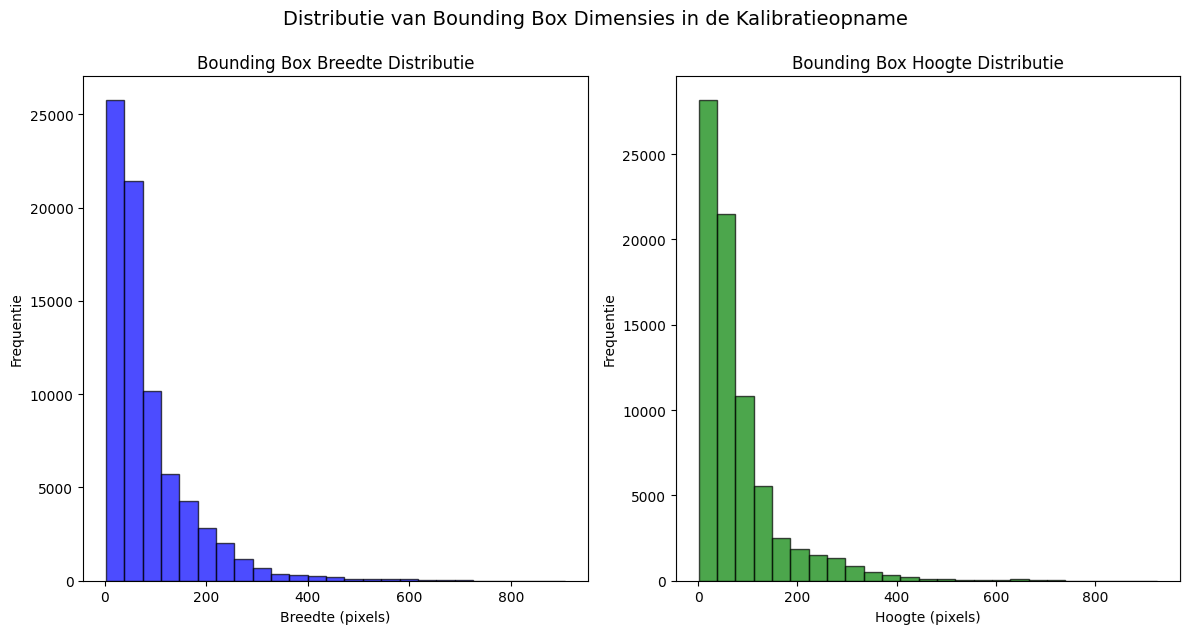
\includegraphics[width=1\textwidth]{bboxes-histogrammen.png}
    \caption[Histogrammen van de breedte en grootte in pixels van bounding boxes in de kalibratieopname]{
      \label{fig:size-histogram}
      Histogrammen van de breedte (links) en hoogte (rechts) in pixels van de bounding boxes in de kalibratieopname.
      De meeste objecten vallen onder de 400 pixels in zowel breedte als hoogte, met een aantal uitzonderingen die groter zijn.
    }
\end{figure}

De volgende overweging betrof de wijze waarop deze crops gegenereerd zouden worden uit de kalibratieopname. 
Aangezien het uiteindelijke doel is om de ROIs die gegenereerd werden door FastSAM, te classificeren, 
dient de trainingsdataset zo goed mogelijk de karakteristieken van deze te classificeren ROIs te weerspiegelen. 
In de praktijk zullen deze ROIs vaak (maar niet altijd perfect) gecentreerd zijn rond het blikpunt van de student, 
omdat de FastSAM-segmentatie en de blikpuntfiltering hierop aansturen. 
Daarom werd voor de creatie van de trainingsdataset besloten om de crops te genereren 
door ze te centreren op het middelpunt van de bounding box van een \textit{geselecteerd doelobject} uit de kalibratieopname. 
Dit simuleert de situatie waarbij het model een ROI aangeboden krijgt waarin het doelobject centraal staat.

Tenslotte vereiste de trainingsdataset voor objectdetectie ook een specifieke structuur, zijnde het 
\textit{Ultralytics YOLO formaat}\footnote{\url{https://docs.ultralytics.com/datasets/detect/\#ultralytics-yolo-format} (laatst geraadpleegd op 2025-05-21).} (zie Codefragment~\ref{fig:yolo-format}).

\begin{listing}[H]
  \begin{minted}{text}
    data/
    ├── images/
    │   ├── train/
    │   │   ├── 0000000001.jpg
    │   │   ├── 0000000002.jpg
    │   │   ├── 0000000003.jpg
    │   │   └── ...
    │   └── val/
    │       ├── 0000000001.jpg
    │       ├── 0000000002.jpg
    │       ├── 0000000003.jpg
    │       └── ...
    ├── labels/
    │   ├── train/
    │   │   ├── 0000000001.txt
    │   │   ├── 0000000002.txt
    │   │   ├── 0000000003.txt
    │   │   └── ...
    │   └── val/
    │       ├── 0000000001.txt
    │       ├── 0000000002.txt
    │       ├── 0000000003.txt
    │       └── ...
    └── data.yml
  \end{minted}
  \caption[Voorbeeld van het Ultralytics YOLO Formaat]{
    \label{fig:yolo-format}
    Voorbeeld van de structuur van de trainingsdataset voor objectdetectie in het Ultralytics YOLO formaat.
    De dataset bestaat uit een map met afbeeldingen (in dit geval crops) en een map met labels.
    Elke afbeelding heeft een bijbehorende labelbestand met dezelfde naam, waarin de bounding boxes en klassen van elk object in de afbeelding zijn gedefinieerd.
    Het data.yml bestand bevat de metadata van de dataset, wat later aan bod komt.
  }
\end{listing}

\subsubsection{Genereren van de Trainingsdataset}

Het eigenlijke proces voor het creëren van de trainings- en validatiedatasets werd gecoördineert door de functie \texttt{create\_dataset} 
(zie Codefragment~\ref{listing:create-dataset-overview}). 
Deze functie neemt de metadata van de gelabelde objecten, de geëxtraheerde frames van de kalibratieopname, 
en configuratieparameters zoals de crop-grootte en het gewenste aantal samples per klasse als input.

\begin{listing}[H]
  \fontsize{10pt}{9.6pt}
  \begin{minted}{python}
  def create_dataset(
      per_class_metadata: dict,
      frames: list[Path],
      datasets_path: Path,
      crop_size: int,
      dataset_type: str,
      num_samples_per_class: int,
  ):
      # Definieren van de paden voor de trainings- en validatiedatasets
      # ... Code weggelaten voor beknoptheid ...

      # Samples selecteren per klasse en train/val splitsen
      selected_samples_per_class = select_samples_per_class(
          per_class_metadata, num_samples_per_class
      )
      all_samples_per_frame = get_samples_per_frame(per_class_metadata)
      train_samples_per_class, val_samples_per_class = get_train_val_split(
          selected_samples_per_class, train_ratio=0.8
      )

      # Datasetfiles aanmaken
      class_label_to_model_id = create_metadata_yaml(dataset_path, per_class_metadata)
      create_train_or_val_dataset(
          per_class_metadata,
          class_label_to_model_id,
          train_samples_per_class,
          all_samples_per_frame,
          frames,
          train_images_path,
          train_labels_path,
          crop_size=crop_size,
      )
      create_train_or_val_dataset(
          per_class_metadata,
          class_label_to_model_id,
          val_samples_per_class,
          all_samples_per_frame,
          frames,
          val_images_path,
          val_labels_path,
          crop_size=crop_size,
          is_validation=True,
      )

      return dataset_path
  \end{minted}
  \caption[Functie voor het creëren van de objectdetectie-trainingsdataset]{
    \label{listing:create-dataset-overview}
    De \texttt{create\_dataset} functie coördineert het creëren van de trainings- en validatiedatasets voor objectdetectie.
    Deze functie definieert de paden voor de datasets, maakt de benodigde mappen aan,
    selecteert de samples per klasse, splitst deze in train- en validatiesets,
    en roept de \texttt{create\_train\_or\_val\_dataset} functie aan om de crops en labels te genereren. 
  }
\end{listing}

De benodigde stappen voor het creëren van de trainingsdataset kunnen worden samengevat in drie hoofdfasen, zoals hieronder beschreven.

\paragraph{1. Verzamelen van Metadata per Klasse}

De notebook laadt in een eerste stap de bestandspaden van de trackingresultaten per klasse 
voor de kalibratieopname via de functie \texttt{get\_tracking\_results\_per\_class} (zie voorgaande Codefragment~\ref{listing:opslaan-segmentatie-resultaten}).
Vervolgens worden op basis van de trackingresultaten, metadata per klasse verzameld door de functie \texttt{get\_metadata\_per\_class} aan te roepen.
Dit resulteert in een dictionary waarin elke klasse ID is gekoppeld aan een dictionary met de volgende informatie:
\begin{itemize}
    \item \texttt{class\_name}: De naam van de klasse, bijvoorbeeld `monitor'.
    \item \texttt{color}: Het kleur van de klasse in hexadecimale notatie.
    \item \texttt{frame\_indexes}: Een lijst van frame-indexen waarin de klasse voorkomt in de trackingresultaten.
    \item \texttt{mask\_areas}: Een lijst van de oppervlakte van het segmentatiemasker voor elk frame waarin de klasse voorkomt.
    \item \texttt{bboxes}: Een lijst van de bounding box voor elk frame waarin de klasse voorkomt.
\end{itemize}
Elke combinatie van een frame-index en bijbehorende bounding box uit deze lijsten representeert 
een uniek gelabeld voorbeeld (een `sample') van een object in de kalibratieopname.

Figuur~\ref{fig:samples-per-class} toont het aantal verzamelde samples per klasse in de kalibratieopname. 
Aangezien sommige objecten dichter bij elkaar stonden, 
zijn er voor die objecten meer samples verzameld dan voor andere.
Zo zien we dat het infuus relatief weinig samples heeft, omdat het in een afgezonderde hoek van het beeld stond.
Hierdoor zijn er enkel samples verzameld binnen de 30 seconden waarin het infuus werd bekeken, 
of wanneer het zichtbaar was in de achtergrond.

\begin{figure}[H]
    \centering
    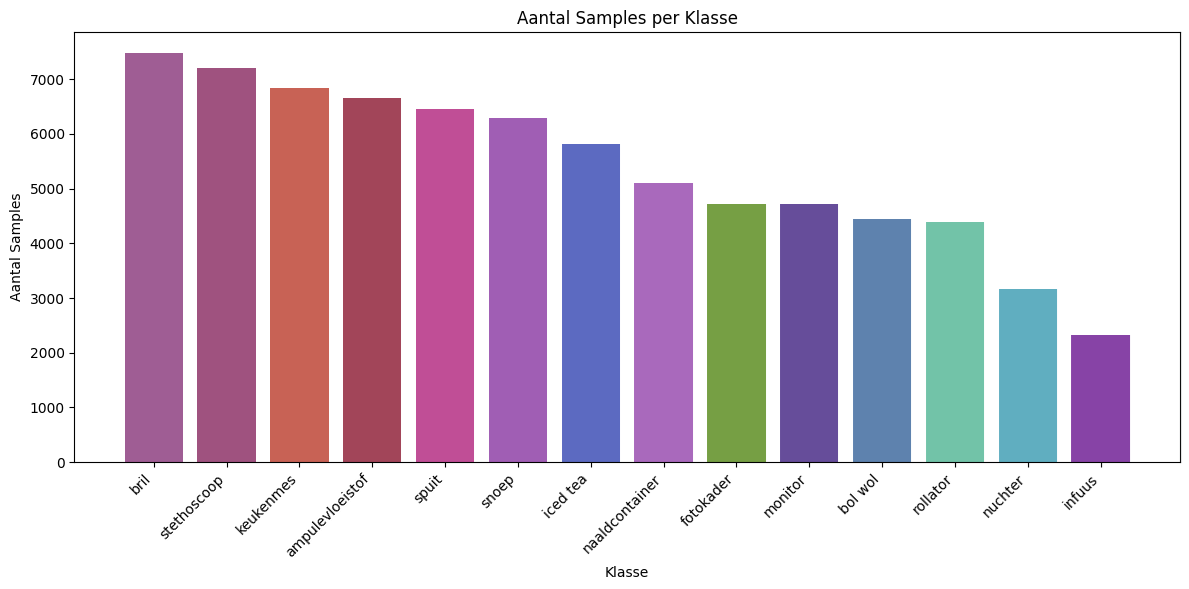
\includegraphics[width=1\textwidth]{samples-per-class.png}
    \caption[Aantal samples per klasse in de kalibratieopname]{
        \label{fig:samples-per-class}
        Aantal samples per klasse in de kalibratieopname.
        De getoonde aantallen zijn het resultaat van de tracking binnen de labeling tool.
      }
\end{figure}

Deze \texttt{per\_class\_metadata} dictionary wordt vervolgens doorgegeven aan de \texttt{create\_dataset} functie.
Elke dataset werd opgeslagen in de map \texttt{data/training\_datasets/object\_detection}.

\paragraph{2. Selectie van Voorbeeldsamples per Klasse}
Om een gebalanceerde dataset te creëren voor training, en om de impact van de datasetgrootte te kunnen onderzoeken, 
werd per objectklasse een specifiek aantal voorbeeld-samples geselecteerd. 
De functie \texttt{select\_samples\_per\_class} implementeert deze selectie. 
Er werd geëxperimenteerd met verschillende aantallen samples per klasse: 500, 1000, 2000 en 3000 via de parameter \texttt{num\_samples\_per\_class}.
Indien een klasse onvoldoende unieke samples bevatte tegenover het opgegeven aantal, werd oversampling toegepast.
Alle beschikbare unieke samples werden eerste geselecteerd, waarna de resterende benodigde samples willekeurig met vervanging ui de beschikbare pool werden getrokken.

Met deze mapping, werden de train- en validatiesets gedefinieerd.
De functie \texttt{get\_train\_val\_split} verdeelt de geselecteerde samples in een train- en validatieset,
met een splitsing van 80\% voor training en 20\% voor validatie.
Deze stap resulteert in twee mappings: \texttt{train\_samples\_per\_class} en \texttt{val\_samples\_per\_class}.

Tenslotte werd ook per frame een lijst van \textit{alle} (dus niet enkel de geselecteerde) bounding boxes verzameld.
Dit is van belang omdat bij het maken van een crop rond een \textit{geselecteerd doelobject},
ook alle \textit{andere} objecten die toevallig in die crop vallen, correct gelabeld moeten worden voor de objectdetector.
De functie \texttt{get\_samples\_per\_frame} creëert hiertoe een dictionary (\texttt{all\_samples\_per\_frame}), 
waarbij elke frame-index gemapt wordt naar een lijst van alle objecten (klasse-ID en bounding box) die in dat frame voorkomen.

\paragraph{3. Genereren van Crops en YOLO-Labels voor Trainings- en Validatiesets}
Met de voorbereide lijsten van geselecteerde trainings- en validatiesamples per 
klasse (\texttt{train\_samples\_per\_class} en \texttt{val\_samples\_per\_class}) 
en de complete lijst van alle gelabelde objecten per frame (\texttt{all\_samples\_per\_frame}), 
kon de daadwerkelijke generatie van de dataset beginnen. 
Dit proces werd uitgevoerd door de functie \texttt{create\_train\_or\_val\_dataset}, 
die afzonderlijk werd aangeroepen voor het creëren van de trainingsdata en de validatiedata. 
De functie \texttt{create\_dataset} fungeerde als een overkoepelende wrapper die de mappenstructuur 
aanmaakte en de \texttt{create\_train\_or\_val\_dataset} functie aanriep (zie Codefragment~{\ref{listing:create-train-val-dataset}}).

% TODO: nederlandse comments + check code page cutoff
\begin{listing}[H]
  \fontsize{11pt}{9.6pt}
  \begin{minted}{python}
    def create_train_or_val_dataset(
      per_class_metadata,
      class_label_to_model_id,
      selected_samples_per_class,
      all_samples_per_frame,
      frames,
      images_path,
      labels_path,
      crop_size: int,
      is_validation=False,
  ):
      selected_samples_per_frame = get_selected_samples_per_frame(
          selected_samples_per_class
      )

      current_sample_idx = 0
      for frame_idx, frame in enumerate(tqdm(frames)):
          # check if the frame has any samples
          if selected_samples_per_frame.get(frame_idx) is None:
              continue

          image = cv2.imread(str(frame))

          # gather boxes and labels for the current frame
          class_ids, bboxes = zip(*all_samples_per_frame[frame_idx])
          bboxes = np.array(bboxes)
          class_labels = [
              per_class_metadata[class_id]["class_name"] for class_id in class_ids
          ]

          # for all selected samples in this frame, create crops
          for _, target_box in selected_samples_per_frame[frame_idx]:
              # create a crop for the current box
              transformed_image, transformed_bboxes, transformed_class_labels = create_crop_for_frame(
                  image,
                  crop_size,
                  target_box,
                  bboxes,
                  class_labels,
                  is_validation
              )

              # Save the transformed image and labels
              create_data_files(
                  labels_path,
                  images_path,
                  class_label_to_model_id,
                  current_sample_idx,
                  transformed_image,
                  transformed_bboxes,
                  transformed_class_labels,
              )

              current_sample_idx += 1
  \end{minted}
  \caption[Functie voor het creëren van de trainings- en validatiedatasets]{
    \label{listing:create-train-val-dataset}
    De \texttt{create\_train\_or\_val\_dataset} functie genereert de crops en labels voor de trainings- of validatiedataset.
    Het laadt de originele afbeelding, verzamelt de relevante bounding boxes en klassenamen,
    en maakt voor elk geselecteerd doelobject een crop rond de bounding box.
    }
\end{listing}

De werking van \texttt{create\_train\_or\_val\_dataset} is als volgt:
\begin{enumerate}
    \item Eerst worden de \texttt{selected\_samples\_per\_class} (die de geselecteerde doelobjecten voor de huidige set bevatten) 
    geherstructureerd naar een per-frame dictionary \texttt{selected\_samples\_per\_frame}.
    \item De functie itereert vervolgens over alle frames van de kalibratieopname.
    \item Voor elke frame wordt de originele afbeelding geladen, indien er samples voor die frame zijn geselecteerd. 
    Ook worden alle bounding boxes en bijbehorende klassenamen van 
    \textit{alle} gelabelde objecten in die frame verzameld uit \texttt{all\_samples\_per\_frame}.
    \item Daarna wordt geïtereerd over elk \textit{geselecteerd doelobject}
    dat in de huidige frame aanwezig is (opgehaald uit \texttt{selected\_samples\_per\_frame}). 
    Het is rond deze \texttt{target\_box} dat een crop zal worden gemaakt.
    \item Voor elk \texttt{target\_box} binnen de frame wordt de functie \texttt{create\_crop\_for\_frame} aangeroepen. 
    Deze functie, hieronder beschreven, retourneert de beelduitsnede, de bounding boxes, en de klassenamen 
    van alle objecten die na het croppen en eventuele augmentatie nog significant zichtbaar zijn binnen die uitsnede.
    \item Tenslotte worden de resultaten opgeslagen via de hulpfunctie \texttt{create\_data\_files},
    die de beelduitsnede en de bijbehorende labels opslaat in de juiste mappenstructuur.
\end{enumerate}

De functie \texttt{create\_crop\_for\_frame} in Codefragment~\ref{listing:create-crop-frame} 
is verantwoordelijk voor het creëren van de crop rond het doelobject.
Het transformeert ook de bounding box-coördinaten van alle relevante objecten naar het coördinatenstelsel van de nieuwe crop,
en past indien nodig augmentaties toe.

% TODO: nederlandse comments + check code page cutoff
\begin{listing}[H]
  \fontsize{12pt}{10pt}
  \begin{minted}{python}
    def create_crop_for_frame(
        image: np.ndarray,
        crop_size: int,
        target_box: tuple[int, int, int, int],
        bboxes: np.ndarray,
        class_labels: list[str],
        is_validation: bool = False,  
    ):
        x1, y1, x2, y2 = target_box
        cx, cy = (x1 + x2) // 2, (y1 + y2) // 2

        # create a crop around the center of the box
        half_crop = crop_size // 2
        x_min = max(0, cx - half_crop)
        y_min = max(0, cy - half_crop)
        x_max = min(image.shape[1], cx + half_crop)
        y_max = min(image.shape[0], cy + half_crop)

        transform_steps = [
            A.Crop(x_min=x_min, y_min=y_min, x_max=x_max, y_max=y_max),
            A.PadIfNeeded(min_height=crop_size, min_width=crop_size),
        ]

        if not is_validation:
            transform_steps.append(A.HorizontalFlip(p=0.5))
            transform_steps.append(A.RandomBrightnessContrast(p=0.2))

        transform = A.Compose(
            transform_steps,
            bbox_params=A.BboxParams(
                format="pascal_voc", label_fields=["class_labels"], min_visibility=0.7
            ),
        )

        # Augment the image and boxes
        augmented = transform(image=image, bboxes=bboxes, class_labels=class_labels)
        transformed_image = augmented["image"]
        transformed_bboxes = augmented["bboxes"]
        transformed_class_labels = augmented["class_labels"]
        return transformed_image, transformed_bboxes, transformed_class_labels
  \end{minted}
  \caption[Functie voor het creëren van een crop rond een doelobject]{
    \label{listing:create-crop-frame}
    De \texttt{create\_crop\_for\_frame} functie maakt een crop rond een doelobject in de afbeelding.
    Het past ook transformaties en augmentaties toe, afhankelijk van of de crop bedoeld is voor training of validatie.
    De functie retourneert de getransformeerde afbeelding, de bounding boxes, en de klassenamen van de objecten in de crop.
    }
\end{listing}

Voor het uitvoeren van beeldtransformaties en augmentaties werd de open-source bibliotheek \texttt{Albumentations} gebruikt \autocite{Buslaev2018}.
De bibliotheek staat toe om eenvoudig transformatiepipelines te definiëren, en vereenvoudigt sterk het werken met bounding-box coördinaten.
Augmentaties kunnen de robustheid van een model verbeteren door extra variatie aan de trainingsdata toe te voegen.
De volgende transformaties en augmentaties werden toegepast:
\begin{itemize}
    \item \textbf{A.Crop}: Deze transformatie werd gebruikt om een vierkante uitsnede te maken rond het geselecteerde doelobject.
    \item \textbf{A.PadIfNeeded}: Soms kan het zijn dat de crop deels buiten de grenzen van de originele afbeelding valt.
    Om dit te voorkomen, wordt padding met nullen toegepast om de crop altijd te vullen tot de gewenste grootte.
    \item \textbf{A.HorizontalFlip}: Deze augmentatie wordt willekeurig toegepast met een kans van 50\% om de afbeelding horizontaal te spiegelen.
    \item \textbf{A.RandomBrightnessContrast}: Deze augmentatie past willekeurig de helderheid en het contrast van de afbeelding aan met een kans van 20\%.
\end{itemize}
De transformaties \texttt{A.Crop} en \texttt{A.PadIfNeeded} worden altijd toegepast,
terwijl de transformaties \texttt{A.HorizontalFlip} en \texttt{A.RandomBrightnessContrast} 
enkel worden toegepast als een crop bedoeld is voor de trainingset (dus niet voor de validatieset).
Het toepassen van de \texttt{A.Crop} transformatie past ook de bounding box coördinaten aan van frame-niveau naar crop-niveau.
Tenslotte heeft de \texttt{A.BboxParams} parameter ook een \texttt{min\_visibility} parameter, die ervoor zorgt dat alleen bounding boxes
met een zichtbaarheid van minstens 70\% worden behouden in de crop.
Deze parameter werd momenteel hardgecodeerd op 70\%, maar kan in de toekomst indien nodig verder geoptimaliseerd worden.

\subsection{Training van YOLOv11 Modellen}

Met de trainingsdatasets aangemaakt, kon de volgende stap beginnen: het trainen van YOLOv11-modellen.
Zoals eerder vermeld, werden vier verschillende datasets gecreëerd, elk met een ander aantal samples per klasse: 500, 1000, 2000 en 3000.
Voor elke datasetconfiguratie werd een afzonderlijk model getraind.

Voor de training werd gebruik gemaakt van het \texttt{YOLOv11n.pt} model. 
Dit is de `nano'-variant van een reeks modellen die zijn voorgetraind op de COCO-dataset \autocite{Khanam2024}.
Het starten met een voorgetraind model is een gangbare praktijk in transfer learning, waarbij het model 
al een basisniveau van kennis heeft over objectherkenning.
Hiermee kan het model sneller convergeren met een kleinere dataset aan domeinspecifieke objecten, tegenover het trainen van een model vanaf nul.

De training werd uitgevoerd met behulp van de functionaliteit van de \texttt{ultralytics} bibliotheek, 
binnen de script \texttt{scripts/train\_object\_detectors.py}.
De relevante code voor het trainen van de modellen is te vinden binnen de functie \texttt{train\_model} in Codefragment~\ref{listing:train-model}.

\begin{listing}[H]
  \begin{minted}{python}
    TRAIN_EPOCHS = 100
    BATCH_SIZE = 0.9
    PATIENCE = 10

    def train_model(dataset_path, model_name, crop_size):
        model = YOLO("yolo11n.pt")

        model.train(
            data=dataset_path / "data.yaml",
            epochs=TRAIN_EPOCHS,
            imgsz=int(crop_size),
            device="cuda",
            batch=BATCH_SIZE,
            patience=PATIENCE,
            plots=True,
            save=True,
        )

        model_path = OBJECT_DETECTION_MODELS_PATH / f"{model_name}.pt"
        model.save(str(model_path))
    }
  \end{minted}
  \caption[Functie voor het trainen van YOLOv11-modellen]{
    \label{listing:train-model}
    De \texttt{train\_model} functie traint een YOLOv11-model op basis van de opgegeven dataset.
    Het gebruikt een voorgetraind model (\texttt{yolo11n.pt}) en traint het op de opgegeven dataset voor een bepaald aantal epochs.
    De \texttt{patience} parameter bepaalt hoeveel epochs het model zonder verbetering mag trainen.
  }
\end{listing}

Voor de training werden de volgende hyperparameters gebruikt:
\begin{itemize}
    \item \textbf{Epochs:} 100 epochs, wat betekent dat het model de volledige dataset 100 keer doorloopt.
    \item \textbf{Batch Size:} 0.9, wat betekent dat de batchgrootte automatisch wordt berekend om 90\% van het beschikbare GPU-geheugen te gebruiken. 
    \item \textbf{Patience:} Een patience van 10 betekent dat de training stopt als er gedurende 10 opeenvolgende epochs geen verbetering in de validatieprestaties wordt gezien.
    Aangezien de prestaties van de modellen tijdens de training echter steeds beter werden tot de 100ste epoch, werd de training niet vroegtijdig gestopt.
\end{itemize}
De \texttt{train\_model} functie werd telkens in een apart proces uitgevoerd voor het beheren van geheugen.
Tenslotte werd elk model opgeslagen in de map \texttt{data/models/object\_detection}.

\subsection{Combineren van Objectdetectie en FastSAM Tracking}

Met de getrainde modellen was het mogelijk om de objectdetectie te integreren met de eerder verkregen FastSAM trackingresultaten uit Sectie~\ref{sec:tracking-segmentatie}.
In deze sectie wordt het proces beschreven om de FastSAM segmentaties te combineren met objectdetectie,
met als doel een dataset te verkrijgen die voor elke frame van de evaluatieopnames een lijst aan gelabelde, bekeken objecten bevat.
Het proces werd geïmplementeerd in de notebook \texttt{13\_predict\_object\_detection.ipynb} en kan worden samengevat in de volgende stappen:
\begin{enumerate}
    \item \textbf{Genereren van Vergelijkingssets per Frame}: Voor elke frame van een evaluatieopname werd een 
    `vergelijkingsset' samengesteld. 
    Deze set bracht de informatie uit twee bronnen samen. 
    De eerste component bestond uit de door FastSAM geïdentificeerde objectsegmenten, 
    die al eerder op basis van de blikdata van de student waren geselecteerd. 
    De tweede component bevatte de objectdetecties die resulteerden uit het toepassen van het getrainde 
    YOLOv11-model op een specifieke uitsnede (crop) van het betreffende frame, 
    waarbij deze uitsnede gecentreerd was rond het blikpunt van de student.
    \item \textbf{Matchen van Segmentaties en Detecties:} 
    Binnen elke vergelijkingsset werden de FastSAM-segmentaties gematcht aan de YOLOv11-detecties op 
    basis van ruimtelijke overlap (Intersection over Union, IoU), waarbij enkel betrouwbare matches werden behouden.
    De term `Intersection over Union' wordt in de volgende sectie verder toegelicht (Figuur~\ref{fig:iou-conceptual}).
    \item \textbf{Toekennen van een Klasse aan FastSAM Object Tracks:} 
    De klassevoorspellingen van de gematchte YOLOv11-detecties werden geaggregeerd voor elke unieke FastSAM object ID 
    (die een object over meerdere frames volgt). 
    Op basis hiervan werd een definitieve classificatie (één van de 14 kritische objecten of 'onbekend') 
    toegekend aan elke FastSAM-track.
    \item \textbf{Samenstellen van de Finale Voorspellingsdataset:} 
    De resulterende, nu gelabelde FastSAM-tracks werden per evaluatieopname geconsolideerd 
    tot een finale voorspellingsdataset, die per frame de geïdentificeerde, bekeken objecten specificeert.
\end{enumerate}
In de volgende sectie worden deze voorspellingsdatasets geëvalueerd tegenover de grondwaarheid, en worden de resultaten besproken.

\subsubsection{Genereren van Vergelijkingssets per Frame}

De eerste stap in het combineren van de FastSAM-trackingresultaten met de YOLOv11-objectdetectie was het per frame samenstellen van een `vergelijkingsset'.
Dit vormde een dataset die later gebruikt zou worden om de finale voorspellingsdataset te creëren.
De functie \texttt{get\_comparison\_dataset} implementeert de logica voor het genereren hiervan (zie Codefragment~\ref{listing:get-comparison-set}).

De volgende functieparameters werden op voorhand samengesteld:
\begin{itemize}
    \item \texttt{frame\_to\_gaze\_position}: Een dictionary die per frame-index het (x,y)-coördinaat van het 
    blikpunt van de student bevat. 
    Deze data werd eerder berekend in Sectie~\ref{sec:synchronisatie-blikpunten-videoframes}.
    \item \texttt{frame\_to\_gaze\_segmentation\_data}: Een dictionary 
    die per frame-index de resultaten van de FastSAM-tracking bevat (bounding boxes en object ID's van de door de blik bekeken segmenten).
\end{itemize}

Vervolgens worden voor elke frame in de evaluatieopname de volgende stappen uitgevoerd:
\begin{enumerate}
    \item Indien er een blikpunt beschikbaar is voor de huidige frame, wordt de afbeelding geladen.
    \item De functie \texttt{create\_frame\_crop} (zie Codefragment~\ref{listing:create-frame-crop}) wordt aangeroepen om een crop te maken rond het blikpunt van de student.
    Deze functie transformeert ook de bounding-boxes van de FastSAM-segmentaties naar het coördinatenstelsel van de nieuwe crop.
    Hier werd net zoals bij de creatie van de trainingsdataset, Albumentation gebruikt om de crop te maken.
    Segmentaties die minder dan 70\% zichtbaar zijn in de crop, werden weggelaten via de \texttt{min\_visibility} parameter.
    \item Het getrainde YOLOv11-model wordt toegepast op de gemaakte crop, en de voorspellingen worden verzameld.
    \texttt{model.predict} aanvaart twee belangrijke parameters:
    \begin{itemize}
        \item \texttt{conf}: De drempel voor de vertrouwensscore van de voorspellingen.
        Deze werd hier ingesteld op 0.5 om in deze stap veel voorspellingen te krijgen. 
        Op deze manier kan later geëxperimenteerd worden met het filteren van voorspellingen bij het matchen van segmentaties en detecties.
        \item \texttt{iou}: De drempel voor de Intersection over Union (IoU) bij het filteren van overlappende voorspellingen.
    \end{itemize}
    \item De resultaten worden opgeslagen in een dictionary met de volgende informatie:
    \begin{itemize}
        \item De FastSAM-segmentatiegegevens (bounding boxes en object ID's).
        \item De YOLOv11-voorspellingen (bounding boxes, klasse-ID's en vertrouwensscores).
    \end{itemize}
\end{enumerate}
Tenslotte worden alle vergelijkingsdatasets voor de verschillende evaluatieopnames opgeslaan als JSON-bestanden in de map 
\texttt{data/comparison\_datasets/<recording\_id>.json}.

% TODO: comments?
\begin{listing}[H]
  \fontsize{10pt}{9.6pt}
  \begin{minted}{python}
    def get_comparison_dataset(
        recording_id: str,
        model: YOLO,
        frame_paths: list[Path],
        frame_to_gaze_position: dict[int, tuple[int, int]],
        frame_to_gaze_segmentation_data: dict[int, dict],
    ) -> None:
        comparison_dataset = {}
        
        for frame_path in tqdm(frame_paths, desc=f"Running inference for {recording_id}"):
            frame_idx = int(frame_path.stem)
            if frame_to_gaze_position.get(frame_idx) is None:
                continue

            image = cv2.imread(str(frame_path))
            gaze_position = frame_to_gaze_position[frame_idx]

            transformed_image, transformed_gs_boxes, transformed_gs_object_ids = create_frame_crop(
                image,
                gaze_position,
                frame_to_gaze_segmentation_data,
                frame_idx
            )

            results = model.predict(
                source=transformed_image, conf=0.5, iou=0.5, device="cuda", verbose=False
            )

            predicted_confidences = []
            predicted_bboxes = []
            predicted_class_ids = []
            for box in results[0].boxes:
                conf = float(box.conf[0].cpu().numpy())
                class_id = int(box.cls[0])
                x1, y1, x2, y2 = box.xyxy[0].cpu().numpy()
                predicted_confidences.append(conf)
                predicted_bboxes.append((int(x1), int(y1), int(x2), int(y2)))
                predicted_class_ids.append(class_id)

            comparison_dataset[frame_idx] = {
                "gaze_segmentation": {
                    "boxes": transformed_gs_boxes.astype(np.int32).tolist(),
                    "object_ids": transformed_gs_object_ids,
                },
                "predicted": {
                    "boxes": predicted_bboxes,
                    "class_ids": predicted_class_ids,
                    "confidences": predicted_confidences,
                },
            }

        return comparison_dataset
  \end{minted}
  \caption[Functie voor het creëren van vergelijkingsdataset voor een evaluatieopname]{
    \label{listing:get-comparison-set}
    De \texttt{get\_comparison\_dataset} functie genereert een vergelijkingsdataset voor een evaluatieopname.
    Deze dataset bevat de FastSAM-segmentaties en de YOLOv11-voorspellingen voor elke frame.
    De functie maakt een crop rond het blikpunt van de student, past het YOLOv11-model toe op deze crop,
    en slaat de resultaten op in een dictionary die per frame de segmentatie- en detectiegegevens bevat.
    }
\end{listing}

% TODO: comments?
\begin{listing}[H]
  \fontsize{12pt}{10pt}
  \begin{minted}{python}
    def create_frame_crop(
        image: np.ndarray,
        gaze_position: tuple[int, int],
        frame_to_gaze_segmentation_data: dict[int, dict],
        frame_idx: int
    ) -> tuple[np.ndarray, list[tuple[int, int, int, int]], list[int]]:
        gaze_segmentation_boxes = frame_to_gaze_segmentation_data[frame_idx]["boxes"]
        gaze_segmentation_object_ids = frame_to_gaze_segmentation_data[frame_idx][
            "object_ids"
        ]

        cx, cy = gaze_position
        x_min = max(0, cx - IMG_CROP_SIZE_HALF)
        y_min = max(0, cy - IMG_CROP_SIZE_HALF)
        x_max = min(image.shape[1], cx + IMG_CROP_SIZE_HALF)
        y_max = min(image.shape[0], cy + IMG_CROP_SIZE_HALF)

        transform = A.Compose(
            [
                A.Crop(x_min=x_min, y_min=y_min, x_max=x_max, y_max=y_max),
                A.PadIfNeeded(min_height=IMG_CROP_SIZE, min_width=IMG_CROP_SIZE),
            ],
            bbox_params=A.BboxParams(
                format="pascal_voc", label_fields=["object_ids"], min_visibility=0.7
            ),
        )

        transformed = transform(
            image=image,
            bboxes=gaze_segmentation_boxes,
            object_ids=gaze_segmentation_object_ids,
        )
        transformed_image = transformed["image"]
        transformed_gs_boxes = transformed["bboxes"]
        transformed_gs_object_ids = transformed["object_ids"]

        return transformed_image, transformed_gs_boxes, transformed_gs_object_ids
  \end{minted}
  \caption[Functie voor het creëren van een crop rond het blikpunt van de student]{
    \label{listing:create-frame-crop}
    De \texttt{create\_frame\_crop} functie maakt een crop rond het blikpunt van de student in de afbeelding.
    Het past ook de bounding boxes van de FastSAM-segmentaties aan naar het coördinatenstelsel van de nieuwe crop.
    Indien een segmentatie minder dan 70\% zichtbaar is in de crop, wordt deze weggelaten.
    De functie retourneert de getransformeerde afbeelding, de aangepaste bounding boxes, en de object ID's van de segmentaties.
    }
\end{listing}

\subsubsection{Matchen van Segmentaties en Detecties}

De volgende stap was het koppelen van de FastSAM-segmentaties aan de YOLOv11-detecties binnen elke vergelijkingsset.
Het doel was om voor elke FastSAM-segmentatie te bepalen welke YOLOv11-detectie, indien aanwezig, het beste overeenkwam.
Aangezien de code veel dataverwerkingsstappen bevat, worden hier enkel de belangrijkste conceptuele stappen beschreven.
De functie \texttt{get\_matched\_boxes\_per\_frame} implementeert de logica voor het matchen van de segmentaties en detecties.
Deze functie aanvaart twee parameters die later binnen een grid-search worden geëvalueerd:
\begin{itemize}
  \item \texttt{min\_pred\_conf}: De minimum vereiste vertrouwensscore voor een YOLOv11-detectie om als geldig te worden beschouwd.
  \item \texttt{iou\_threshold}: De minimum Intersection over Union (IoU) drempel die vereist is om een match te beschouwen als geldig.  
\end{itemize}
IoU wordt gedefinieerd als de verhouding tussen de oppervlakte van de overlap tussen twee bounding boxes en de oppervlakte van hun unie.
Zie Figuur~\ref{fig:iou-conceptual} voor een visuele representatie van IoU.

\begin{figure}[H]
    \centering
    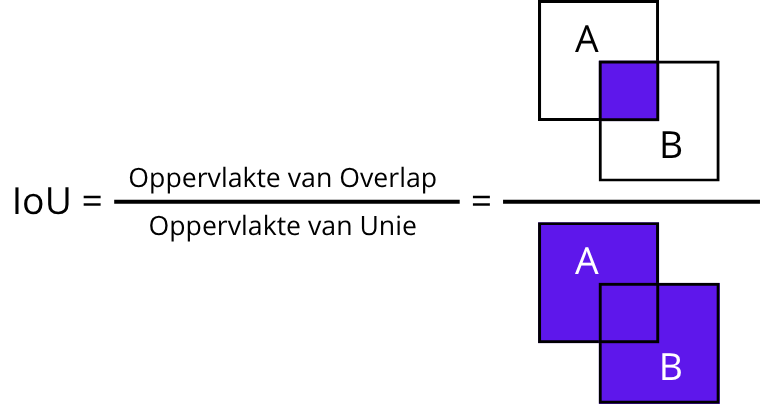
\includegraphics[width=0.6\textwidth]{iou_conceptual.png}
    \caption[Conceptuele weergave van Intersection over Union (IoU)]{
        \label{fig:iou-conceptual}
        Conceptuele weergave van Intersection over Union (IoU).
        De overlap tussen de twee rechthoeken wordt gedeeld door de unie van de twee rechthoeken.
        Dit resulteert in een waarde tussen 0 en 1, waarbij 1 betekent dat de rechthoeken volledig overlappen.
        (eigen afbeelding)
      }
\end{figure}

De matching-functie omvat de volgende conceptuele stappen:
\begin{enumerate}
    \item Voor elke frame in de vergelijkingsset worden de FastSAM-segmentaties en YOLOv11-detecties opgehaald.
    \item De objectdetectie-voorspellingen worden gefilterd op basis van de \texttt{min\_pred\_conf} parameter.
    \item Indien er voor een klasse meerdere detecties zijn, wordt enkel de detectie met de hoogste vertrouwensscore behouden.
    \item Indien er geen voorspellingen overblijven na filtering, wordt de frame overgeslagen.
    \item Voor elke FastSAM-segmentatie wordt de IoU berekend met elke geldige YOLOv11-detectie.
    \item Indien de IoU groter is dan de \texttt{iou\_threshold}, wordt de detectie beschouwd als een match voor de segmentatie.
    \item Voor elke segmentatie wordt de beste match bepaald op basis van de hoogste IoU.
    \item Tenslotte wordt de lijst van gematchte segmentaties, detecties en hun IoU-waarden opgeslagen in een dictionary per frame.
\end{enumerate}

\subsubsection{Toekennen van een Klasse aan FastSAM Object Tracks}

Na de matchingstap beschikken we per frame over een lijst van FastSAM-segmentaties die 
succesvol gekoppeld konden worden aan een YOLOv11-objectdetectie.
De volgende uitdaging is om op basis van deze per-frame informatie, een definitieve klasse toe te kennen aan elke unieke FastSAM object ID
die doorheen de evaluatieopname werd gevolgd.
Een object ID kan immers over meerdere frames worden waargenomen, 
en het YOLOv11-model kan in verschillende frames verschillende voorspellingen doen voor hetzelfde object (of zelfs geen voorspelling doen)
De aggregatie dient de ruis van individuele voorspellingen te reduceren.

Dit proces, inclusief de vorige matchingstap, werd geïmplementeerd in de overkoepelende functie \texttt{get\_predictions\_df}.
De belangrijkste conceptuele stappen zijn als volgt:

\paragraph{1. Aggregeren van Voorspellingen per FastSAM Object ID}
De eerste stap is het verzamelen van alle YOLOv11-klassevoorspellingen en hun bijbehorende 
vertrouwensscores die gematcht zijn met een specifieke FastSAM object-ID, 
ongeacht in welke frame ze voorkwamen. 
Dit aggregeert de per-frame matchresultaten naar een lijst van voorspellingen voor elke unieke getrackte entiteit. 
De functie \texttt{get\_predictions\_per\_object\_id} voert deze groepering uit en genereert een dictionary waarin elke FastSAM object-ID is gekoppeld aan een lijst van voorspellingen.
Voor elke voorspelling wordt de klasse-ID en de bijbehorende vertrouwensscore opgeslagen.

\paragraph{2. Filteren op Minimale Observatieduur}
In de evaluatiestap werd er ook onderzocht of het zinvol was om een parameter te introduceren die bepaalt hoeveel frames een object moet worden waargenomen
voordat het wordt geclassificeerd. Dit zou eventueel een effect hebben op vals-positieve voorspellingen, omdat korte ovservaties meer vatbaar zijn voor ruis.
Zo worden enkel object tracks die in minstens een bepaald aantal frames zijn waargenomen, behouden.
Dit wordt aangedreven door de parameter \texttt{min\_observed\_frames} in de functie \texttt{filter\_by\_min\_observed\_frames}.

\paragraph{3. Toekennen van de Finale Klasse per Track}
Voor elke overgebleven FastSAM object-track, wordt nu één definitieve klasse bepaald door de functie \texttt{get\_final\_prediction\_per\_object\_id}. 
Hier wordt voor elke object ID de klasse gekozen die de hoogste totale som van YOLOv11-vertrouwensscores 
behaalde over de gehele duur van de track. 
Dit kan gezien worden als een vorm van stemmingsaggregatie, 
waarbij de klasse met de meeste `stemmen' (in termen van vertrouwensscores) wordt gekozen.

\subsubsection{Samenstellen van de Finale Voorspellingsdataset}
Het resultaat van de vorige stap was een mapping van FastSAM object-ID's, 
naar hun definitieve voorspelde klasse (één van de 14 kritische objecten) 
en de geaggregeerde vertrouwensscore.
In Sectie~\ref{sec:voorbereiding-tracking-resultaten} werd al beschreven hoe de metadata van de FastSAM-trackingresultaten opgeslagen werden in zogenaamde `object-datasets'.
In deze stap werden deze datasets, voor elke evaluatieopname, uitgebreid met de voorspelde klasse en de bijbehorende vertrouwensscore voor elke object ID.
Het resultaat was een finale voorspellingsdataset per evaluatieopname die klaar was voor evaluatie en de volgende velden bevatte:
\begin{itemize}
    \item \texttt{frame\_idx}: De index van de frame in de evaluatieopname.
    \item \texttt{object\_id}: De unieke ID van het getrackte object.
    \item \texttt{gs\_confidence}: De vertrouwensscore van de FastSAM-segmentatie voor het object in de frame (dus niet van de YOLOv11-detectie).
    \item \texttt{mask\_area}: De oppervlakte van de FastSAM-segmentatie in pixels.
    \item \texttt{x1, y1, x2, y2}: De coördinaten van de bounding box van de FastSAM-segmentatie in de frame.
    \item \texttt{predicted\_class\_id}: De voorspelde klasse-ID van het object, gebaseerd op de YOLOv11-detecties.
    Indien er geen voorspelling was voor het object, werd deze op -1 gezet (dit betekent dat het object als `onbekend' wordt beschouwd).
    \item \texttt{predicted\_confidence}: De geaggregeerde vertrouwensscore van de voorspelde klasse, gebaseerd op de YOLOv11-detecties.
\end{itemize}

\section{Evaluatie van de Analysepipeline}

\section{Samenvatting van de Gehele Analysepipeline}